% Chapter 1

l\chapter{Introduction} % Main chapter title

\label{Introduction} % For referencing the chapter elsewhere, use \ref{Chapter1} 

%----------------------------------------------------------------------------------------

% Define some commands to keep the formatting separated from the content 
\newcommand{\keyword}[1]{\textbf{#1}}
\newcommand{\tabhead}[1]{\textbf{#1}}
\newcommand{\code}[1]{\texttt{#1}}
\newcommand{\file}[1]{\texttt{\bfseries#1}}
\newcommand{\option}[1]{\texttt{\itshape#1}}

%----------------------------------------------------------------------------------------

\section{Modern Cosmology}
 
\subsection{The Big Bang Theory}
The basis for modern cosmology relies on several fundamental assumptions stemming from observation, the chief of which is the Big Bang Model. Following Hubble's discovery of a relation between distances to galaxies and their recessional velocities, the \emph{Copernican Principle} leads to the conclusion that in the past, objects in the universe were much closer together. His observations gave rise to the Lemaitre's Hubble Law, 
\begin{equation}
v  \varpropto d 
\label{eq:HubbleLaw}
\end{equation}
This suggests that at some point in the past, the universe was much smaller than it is at present, the conservation of energy then implies that at some point in the past, the universe must have been an incredibly hot, dense environment. Using general relativity, the extrapolation backwards in time yields a singularity of infinite density and temperature, which is commonly called the \emph{Big Bang}
\par Another assumption stemming from observation is that of isotropy. Based on observation, there appears to be no favoured direction in the universe, since distributions of distant galaxies and other extragalactic sources seem to be evenly distributed across the sky. Perhaps the most spectacular example of this isotropy is the presence of the \emph{Cosmic Microwave Background}. 
\par Discovered in 1964 \citep{Penzias:65}, it was noticed that there was isotropic black-body radiation at $T \approx \SI{2.7}{\kelvin}$. Since the peak of this radiation is in the microwave section of the electromagnetic spectrum, it was termed the \emph{Cosmic Microwave Background}. 
\begin{figure}[ht]
\centering
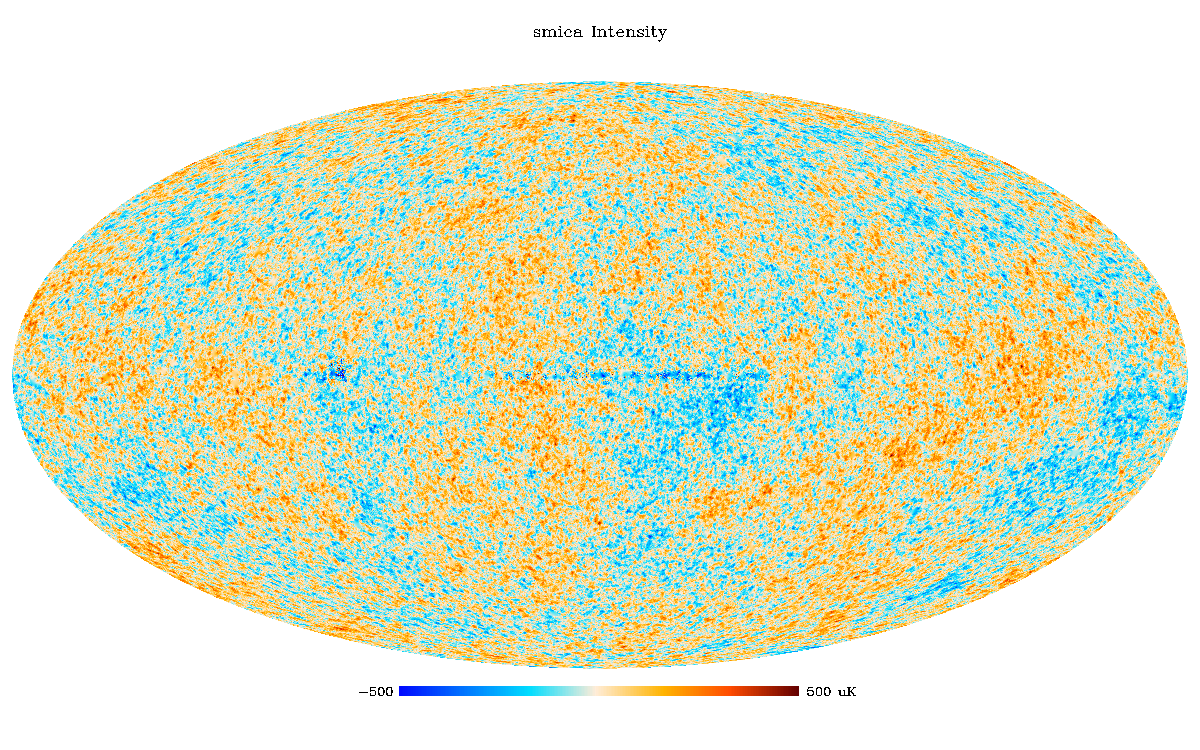
\includegraphics[scale=0.25]{../Images/CMB_smica_tsig.png} 
\label{CMB Map}
\caption{\emph{Planck} Satellite Full Sky CMB Map}
\end{figure}
This reflects the Big Bang Model, which suggests that space is filled with radiation left over from the initial singularity, and is reinforced by the fact that the background light has a flux orders of magnitude greater than other emitting sources.
\par This picture of the Big Bang, whilst useful at a basic level, presents problems when examined more closely. As it stands, the edges of the observable universe at present are too far away from each other to be causally connected. What accounts for the observed homogeneity and isotropy then, if entire areas of the universe cannot affect each other, or communicate information, and so cannot mix? Measurements of the CMB also indicate that the universe is spatially flat, but the initial conditions required to maintain this state are incredibly specific. There is no reason to suggest that these conditions should be preferentially selected over any others. If the conditions for homogeneity and isotropy are maintained sufficiently to allow this, how then does the observed large scale structure of the universe come about? There are also addition problems arising from particle physics, including considerations regarding magnetic monopoles and gravitinos, which have to be satisfied.

\subsection{Inflation}
The most commonly held solution to these problems is the theory of \emph{cosmological inflation}\cite{Linde:07}. This is a period at a very early epoch of the universe where the expansion rate of the universe is exponentially large. This expansion allows to patches of the universe to be causally connected to each other at early times, as well as flatten out as it evolves, effectively solving the issues of precise tuning with one soluton.

Inflation is driven by an energy field, known as the \emph{inflaton field}. When we treat this field from a quantum mechanical perspective, we observe little lumps of uncertainty in a univorm background appear. As the universe expands, these pockets of uncertainty go from being virtual and mathematical to real and physical. As it expands further, these grow into classical objects, such as galaxies, stars, and the other hallmarks of anisotropy we observe. 

This expansion allows for random fluctiations origininating on the quantum scale to grow into macroscopic ones, whilst still maintain their causal connection at very early times. It therefore allows us to explain large scale regularity and small scale irregularity with the same model. 

The simplest mechanism proposed invokes a scalar field, which we loosely couple to gravity using the equation 
\begin{equation}\label{eq:sclr_inf}
\ddot{\phi} + 3 H \dot{\phi} + V^\prime(\phi) = 0
\end{equation}

The conditions for inflation arise from the Friedmann Equations, and the requirement that the fluctuations grow more rapidly than the characteristic scale on which events are causally connected. 

This manifests as an explcit relation between the pressure gradient of the universe, and its density
\begin{equation}\label{eq:inf_cndtn}
3 P < \rho
\end{equation}
which in turn is satisfied by a \emph{slow-roll} field, whereby 

\begin{equation}\label{eq:slw_rll}
\dot{\phi}^2 < V
\end{equation}
Practically, all the proposed models satisfy three conditions \cite{LiddleLyth:00}. Firstly, the 'force' of the time-varying potential $V^\prime$ balances against the frictive term $3 H \dot{phi}$, which makes the field's motion overdamped. This corresponds to the mathematical relation
\begin{equation}\label{eq:slw_rll_cond1}
\dot{\phi} \simeq - \frac{1}{3 H} V^\prime
\end{equation} 
Secondly, in order to satisfy \ref{eq:slw_rll}, we introduce a parameter $\epsilon$ 
\begin{equation}\label{eq:slw_rll_cond2}
\epsilon \equiv \frac{m_{Pl}^2}{16 \pi} \left(\frac{V^\prime}{V}\right)^2 << 1
\end{equation}
This also leads to the following expression
$$ H^2 \simeq \frac{1}{3} \frac{8 \pi}{m_{Pl}^2} V $$
These together imply that the scale factor, the measure of the rate of expansion of the universe, grows approximately exponentially
$$a \propto e^{Ht} $$
The third condition can be derived from the other two, by differentiation the approximation \ref{eq:slw_rll_cond1}, and maintaining consistency with \ref{eq:sclr_inf}. This third condition is technically independant from the other two however, since there is no requirement that the derivative of an approximation to itself be a valid approximation. 
\begin{equation}\label{eq:slw_rll_cond3}
|\eta| \equiv \left| \frac{m_{Pl}^2}{8 \pi} \frac{V^{\prime \prime}}{V} \right| << 1 
\end{equation}
These conditions are necessary, but are not sufficient, since they only specify conditions of the inflation field, not the form of the field itself, due to the field being subject to a second order scalar wave equation. 

Inflation is a powerful tool to solve theoretical problems, however we lack direct confirmation of its mechanism. Particle physics is currently agnostic on direct detection of particles created by the field, and so we must search for tracers elsewhere. 

\subsection{Inflation and Gravitational Waves}
Regardless of the precise model of inflation, all models predict that the period of rapid expansion would have produced primordial gravitational waves, being produced as a vacuum fluctuation in the same way as the density fluctuations. 

\par In the Friedmann-Robertson-Walker Universe, a gravitational wave corresponds to a spatial metric perturbation. Due to general relativity, the gravitational waves that arise in the inflationary period will remain constant until they enter the horizon (where they have a scale comparable to the size of the universe), before they start to vary. It is only well after they enter the horizon, that they will start to decay, which corresponds to the graviational waves redshifting with the expansion of the universe. 

\par This means that the corresponding contributions of the primordial gravitational waves will be to the low multipole anisotropy at $l<<100$, since these are the only modes that aren't redshifted away when the CMB decouples. 

\par The effect these gravitational waves has on the CMB is incredibly difficult to detect in the temperature of the CMB, since they are almost negligible when compared to the density perturbations. However, luckily, the effects of primordial graviational waves can be found in the polarization of the CMB. 

\par The CMB is to predicted to have a relatively low level (roughly ~10\%) of linear polarisation resulting from Thompson scattering as it emerges from the surface of last-scattering, as well as some polarisation after reionization. If we recall the classical description of polarized electromagnetic radiation, we can consider a plane wave's electric field arriving from the $+z$ directin to be described by Fourier components
\begin{align*}
E_x (t) &= E_x \cos(\omega t - \delta_1) \\
E_y (t) &= E_y \cos(\omega t - \delta_2)
\end{align*} 

From these, we can write down the frequency average of the CMB as being an ensemble average of each Fourier component
$$ 4 \frac{\text{intensity}}{d \omega} = 4 \left< E_{pol}^2 \right> =  I + Q \cos(2 \phi_{pol}) + U \sin(2 \phi_{pol}) $$
Where 
\begin{align*}
I &= \left< E_x^2 + E_y^2 \right> \\
Q &= \left< E_x^2 - E_y^2 \right> \\
U &= \left<2 E_x E_y \cos(\delta_1 - \delta_2) \right> \\
\phi_{pol} &= \text{The Angle of Polarisation around the x-axis }\\
& \text{clockwise around the z-axis}
\end{align*}

These ($I,Q,U$) are known as the Stokes Parameters, and can be directly detected through the use of clever multi-chroic dual-polarization bolometric detectors \cite{1210.8256}. Since our choice of direction is arbitrary over the whole sky, we can define a polar direction carefully, so that 
\begin{align*}
E_\textbf{k} &\equiv Q_\textbf{k} \\
B_\textbf{k} &\equiv U_\textbf{k}
\end{align*}


\par These Stokes Parameters are affected differently, depending on the types of modes generated prior to recombination, and so will be senestive to inflationary physics. The reason for this is that there are three different types of perturbations in the universe, and they do not all couple to each other. Each type, scalar, vector, and tensor perturbations, obey a separate set of linear equations, and so can be considered separately. 

\subsubsection{Scalar Perturbations}
The most common types of perturbations are scalar modes, which are indicative of the energy density of the fluid prior to recombination. These modes form as a result of gravitational instability, and are responsible for large scale structure. They are commonoly thought to be a result of the vacuum fluctutaion of the inflaton field, and its subsequent adiabatic perturbations, with some possiblitiy of other non-inflaton fields, such as the axion and its isocurvature pertubations, contributing to the scalar modes. 

The polarisation pattern that is created as a result of the scalar perturbations is driven by Thompson scattering at the last scattering surface. Due to the orthogonality of the spherical harmonics, the linear polarization of the CMB due to scalar perturbations will reflect the $m=0$ quadrupole, and so have azimuthal symmetry with maximum power in the E and B fields at the equator \cite{Hu:Polarisation}. 

\subsubsection{Vector Perturbations}
Vector Perturbations correspond to vorticies in the primordial fluid, analgous to eddies in a water current, and they lack an assosciated density perturbation. This motion is not enhanced by gravity, so any inital vorticies introduced to the primordial fluid will have their power effectively damped away by the expansion of the universe, since there is no meaningful mechanism to provide power to these modes. 

Despite being damped away, the corresponding temperature fluctuations don't decay away once generated. The Thompson scattering transforms the quadrupole temperature anisotropy into a local polarization field as above, however the quadrupole that applies is the $m=\pm 1$, so the polarisation will be rotated with azimuthal angle, and maximum power at the equator \cite{Hu:Polarisation}.

\subsubsection{Tensor Perturbations}
Tensor Perturbations are transverse-traceless fluctuations in the metric, and so are only created by gravitational waves. A plane gravitational wave 'str\-etch\-es' spacetime in the plane of the perturbation in a quadrupole structure. This is self- evident from General Relativity, where a ring of test particles in the plane of a gravitational wave will be distorted into an ellipse.

The tensor perturbations correspond to the $m=\pm 2$ quadrupole, so they are maximised at the poles, and minimised at the equator. This produces patterns which are technically distinct from the vector and scalar perturbations discussed above \cite{Hu:Polarisation}.

\par Although they separate cleanly by their $m$ values for a single spatial frequency mode, there will in general exist a spectrum of fluctuations, depending on the spatial scale being considered, since we expect the averaged power of each multipole $l$ to be independant of its $m$ value.

\subsubsection{Polarisation}
Any polarization pattern can be separated out into its component $E$ and $B$ modes, which is useful for detecting and measuring the polarisation. The Stokes Parameters that define the $E$ and $B$ modes are defined in a frame-dependant way, since they depend on the reference system at the point of measurement. They take the form of a scalar ($E$) and pseudo-scalar ($B$) field on the surface of a sphere (since the quadrupole gives them an even and an odd parity respectively). From this, we can completely express the polarization and temperature of the CMB with four quantites $C_l^{TT}$,$C_l^{TE}$,$C_l^{EE}$, and $C_l^{BB}$, defined by the relation
\begin{equation} \label{eq:cmb_plr_tmp}
C_l^{XY} = \left< a_{lm}^X a_{lm}^{Y\dagger} \right> = \begin{pmatrix}
C_l^{TT} & C_l^{TE} & 0 & 0 \\
C_l^{TE} & C_l^{EE} & 0 & 0 \\
0 & 0 & C_l^{BB} & 0 \\
0 & 0 & 0 & 0
\end{pmatrix}
\end{equation}

\par One thing which must be considered is that the presence of foregrounds and lensing potentials act to shear $E$ modes produced at the surface of last scattering into $B$ modes. This means that in order to actually detect primordial $B$ modes, a detailed model must first be produced for the large scale structure between the CMB and the detector, so that this shearing effect can be taken into account. 

\subsection{Experimental Detection}

\subsubsection{Sensitivity}
One of the primary issues with measuring the CMB Polarisation is that it requires orders of magnitude better instrument sensitivity than the CMB anisotropies. Because the physical detectors are largely already noise limited, it becomes decrease the noise statistically, either by scaling up the number of detectors in an experiment, or increasing their integration time. 

Current experiments are only just currently getting to the down to the senestivity required to detect these B modes  \cite{1412.0626} \cite{1307.5830} \cite{1403.2369}, which do work to give a constraint on the amplitude of lensing, however they do not have adequate signal to noise to successfully separate the primordial $B$ modes from the lensed ones. Some teams have attempted to bring this down by taking cross correlations between experiments \cite{1502.00612}, however the mismatch in systematics between experiments makes this a difficult task. The \textit{Planck} Satellite has provided the most comprehensive all sky maps of the temperature and polarisation of the CMB to date \cite{1807.06205}, and their data does not lead to a detection of a non-zero tensor amplitude \cite{1807.06211}. 

\par In order to address this, a series of experiments have been proposed, called CMB Stage 4 (CMB-S4), whose primary goal is the map the CMB polarisation signal to nearly the limit set by cosmic variance on the angular scales possible from ground based experiments \cite{1610.02743}. Given that the optimum experimental set-up has not yet been determined, it is the hope that utilising a range of existing and promising technologies, as well as separate processing pipelines will allow for errors to be corrected for, and so reduced. CMB-S4 plans to scale up the number of elements, frequency, and bandwidth relative to current instruments. 

\par Small apeture experiments, such as the BICEP/SPIDER/KECK array, or ABS, plan to use cryogenic optics, which hopes to reduce detector noise due to the optical loading in the telescope itself. Operating with apetures less than $~ 1 m$, they will be sensetive to $B-$ mode signals at large angular scales ($l<200$), but not to the lensing signal at higher multipoles. 

\par Large apeture designs, such as the Simmons Array, and SPT-3G, contrast with the small apeture designs by conducting simultaneous observations of multiple frequency bands at apetures of $\gtrsim 1 m $, which allows them to measure the lensing signal at high multipoles ($l>200$). Even larger designs are sensitive to the Sunyaev-Zeldovich effect produced in galaxies and galaxy clusters, which will provide a very good redshift independant tracer for large scale structure \cite{math/0208192} 

\par Overall, the Stage 4 experiments aim to measure the tensor-to-scalar ratio to $\sigma(\textbf{r}) = 0.001$, with an appropriate level of systematic uncertainty \cite{1309.5381}. With this level of uncertainty, a Stage 4 experiment should be able to detect tensor modes at a $5\sigma$ confidence level, from any inflationary model with a $\textbf{r}\gtrsim 0.01$, or simillarly rule out large field inflation with a null detection. The hypothetical limits of Stage 4 experiments should be able to make a measurement of the tensor spectral index $n_t$ at a signal to noise level of $~2$ with a half sky survey and $~1 \mu K$-arcmin noise level.  

\subsubsection{Foregrounds}
In the CMB, there is a window in the electromagnetic spectrum for which the CMB dominates over foregrounds for a significant fraction of the sky. For the most part, the near-independance of the emission of these foregrounds with respect to sky coordinates makes component separation feasible. 

For polarisation however, the situtaion is not as clear. For low frequencies, Faraday rotation makes it difficult to constrain the model of emission. For all frequencies, when you integrate over polarised emission from foregrounds, it averages the polarisation, which gives spatial coherence to the polarisation direction. This directly contrasts to the intensities, which add up provided the emitter is optically thin, which leads to different spectra for the polarisation and the intensity power spectra for foregrounds.

In order to combat this, multiple frequency experiments which are extremely sensetive are required in order to accurately measure the foregrounds. Such experiments allow for one to check that polarisation has the expected form of the derivative of a black-body emission law. 

\subsection{Map Making for Next Stage Experiments}
Achieving the science goals for the next generation of CMB experiments requires careful survey construction and experimental design. Measuring the tensor-to-scalar ratio to an appropriate level requires mapping at minimum, hundreds of square degrees of the sky, to noise levels below $\SI{10}{\micro\kelvin}$ in a 1-arcmin pixel resolution. If we want to effectively clean out lensing foregrounds from the $B$ modes, we have even further restrictions on sensitivity. Delensing to any significant degree requires a beam size less than 10 arcmin, and less than $\SI{5}{\micro\kelvin}$ \cite{0811.3915}. This resolution and noise level across a $\SI{1000}{\deg^2}$ would reduce the limit on the measurement of $r$ due to lensing to $10^{-3}$.

\par A Stage 4 polarisation experiment must be designed with some key features. It must have multiple frequency bands, so as to separate polarised foreground signals. It must be sensitive on arcminute scales to effectively delense the signal, as well as being sensitive on degree scales to observe the primordial tensor mode signal. It clearly must have low noise from an optical and instrumental standpoint, so as to reduce the likelihood of false polarisation signals, and a balance must be found between the integration time and the map size. According to te \textit{Planck} Sky model, for each fraction of sky covered, the cleanest frequency in terms of foregrounds will sit at $\SI{95}{\giga\hertz}$. 

\par There is an expected 'recombination bump' at a characteristic scale of $\Theta ~ 2\deg$, which corresponds to a multipole of $l ~ 100$. According to theoretical predictions, this bump will dominate over lensing as very large angular scales ($l<10$), even for low values of $r$, however galactic dust predictions at these scales are expected to be a factor of 30 larger.

\par Since lensing induced $B$ modes have the same frequency dependance as the CMB, they cannot be distinguished by multi-frequency observations. The lensing peaks at $l ~1000$, so it will drive the survey towards increasing its width, because covering more sky will allow for lensing confusion to subtracted in power-spectrum space (\textit{debiasing}) in the same way instrumental noise is corrected for in temperature power spectrum experiments. Alternatively, the lensing deflection field can be reconstructed from high resolution arcminute scale measurements of the $B$ modes, and can be subtracted away from lower resolution degree scale $B$ mode maps to give the primordial signal. This process however, necessitates larger apeture telescopes.

\par The method of map-making utilised by the majority of CMB experiments is outlined by Tegmark in \cite{astro-ph/9705188}, and by Hivon in \cite{astro-ph/0105302}, however, the unique design of each experiment requires these processing pipelines to be built independantly for each experiment. 

